\documentclass{article}
\usepackage[utf8]{inputenc}
\usepackage{amsfonts}
\usepackage{geometry}
 \geometry{
     a4paper,
     total={165mm,257mm},
     left=25mm,
     top=20mm,
 }

\usepackage{graphicx}
\usepackage{caption}
\usepackage{epsfig}
\usepackage{subfig}
\usepackage{float}
\usepackage{hyperref}
\hypersetup{
    colorlinks=true,
    linkcolor=blue,
    filecolor=magenta,
    urlcolor=cyan,
}

\title{Rapport Python3}
\author{Ewald Janin }
\date{Dernière mise à jour : 24 Mai 2020}

\usepackage{natbib}

\begin{document}

\maketitle

\section{Étude théorique}


\subsection{Influence du taux d'apprentissage $\eta$}

La formule de calcul du delta à appliquer sur le vecteur poids pour le mettre à jour pour chacun des neurones est $\Delta W_j = \eta e^{-\frac{||j-j^*||^2_c}{2\sigma^2}}(X-W_j)$.
\\Dans le cas présent, nous étudions le neurone gagnant, donc $||j-j^*|| = 0$, ce qui nous donne $e^{-\frac{||j-j^*||^2_c}{2\sigma^2}} = 1$ (car $\forall x \in \mathbb{R}, x^0 = 1$). On peut donc ramener la formule de calcul de la mise à jour du poids à $\Delta W_j = \eta (X-W_j)$.

\subsubsection{Cas taux d'apprentissage $\eta = 0$}

Dans le cas où $\eta = 0$, nous identifions immédiatement que $\Delta W_j = 0$. Il n'y a donc pas de modification appliquée sur le vecteur poids de chacun des neurones, donc leur poids restera celui qui a été déterminé à l'initialisation.

\subsubsection{Cas taux d'apprentissage $\eta = 1$}

Dans le cas où $\eta = 1$, $\Delta W_j = (X-W_j)$, c'est à dire que le delta de mise à jour pour le poids est égal à la distance euclidienne entre le neurone et l'entrée, donc son nouveau poids est la valeur de l'entrée : $W = W^* + (X-W^*) = X$.

\subsubsection{Cas taux d'apprentissage $\eta \in  ]0,1[$}

Dans ce cas là, la formule permettant de calculer le nouveau poids du noeud gagnant est $W_j = \eta X + (1-\eta) W^*$. Cette fonction a pour représentation mathématique un plan. Plus $\eta$ se rapproche de 1, plus le nouveau poids du noeud sera proche de la valeur de l'entrée $X$. À l'inverse, plus $\eta$ tend vers 0, plus le poids va rester similaire à son ancien poids.
\\En résumé, si je note $W_j$ le nouveau poids du noeud gagnant :
\begin{itemize}
    \item $\lim_{\eta \to 0} W_j = W^*$
    \item $\lim_{\eta \to 1} W_j = X$
\end{itemize}
Pour les noeuds voisins, nous obtenons le même résultat, qui est à multiplier par la valeur de la fonction de voisinage, dont les valeurs ici appartiennent à $]0,1[$ pour les noeuds voisins du gagnant. L'influence du taux d'apprentissage $\eta$ est donc la même concernant la composante qui va avoir le plus d'importance dans le calcul du nouveau poids, à ceci près que le noeud apprend moins que le noeud gagnant.


\subsection{Influence de la largeur du voisinage gaussien $\sigma$}

Nous nous replaçons dans le cas général et non plus seulement sur le noeud gagnant, il nous faut donc bien prendre en compte la fonction de voisinage $V(j,j^*) =  e^{-\frac{||j-j^*||^2_c}{2\sigma^2}}$.

\subsubsection{Influence de $\sigma$ sur l'apprentissage des noeuds voisins}

Ici, la fonction de voisinage renvoie une valeur comprise dans $]0,1]$ (car $\lim_{x \to - \infty} e^x = 0$), même si la valeur de 1 n'est retournée que pour le noeud gagnant. Plus les noeuds sont situés loin du noeud gagnant, plus la valeur de cette fonction de voisinage est faible et moins le noeud apprend.
L'augmentation du coefficient de voisinage $\sigma$ va permettre aux noeuds voisins d'apprendre plus, car l'exposant de l'exponentiel aura une valeur plus proche de zéro, et donc la fonction de voisinage sera plus élevée.


\subsubsection{Influence de $\sigma$ sur la densité de l'auto-organisation}

Plus le coefficient de voisinage $\sigma$ est élevé, plus des noeuds plus éloignés du noeud gagnant sont quand même influencés par la valeur de l'entrée du pas courant. Les noeuds vont donc avoir tendance à rester 'proches' les uns des autres avec l'augmentation de $\sigma$.


\subsubsection{Mesure de l'influence de $\sigma$}

Pour mesurer l'influence du coefficient de voisinage $\sigma$, je propose de faire plusieurs simulations avec le même jeu de données et le même réseau de neurones, avec un $\sigma$ variant de très élevé à très bas. Pour mettre ce phénomène le plus en avant possible, nous pourrions utiliser un petit réseau de neurones par rapport aux données, ce qui permettrait de mettre encore plus en évidence la différence de densité du réseau de neurones à convergence.


\subsection{Influence de la distribution d'entrée}

Nous allons maintenant étudier le cas d'un neurone unique recevant deux entrées $X_1$ et $X_2$ présentées un grand nombre de fois chacune, avec un taux d'apprentissage $\eta$ faible.

\subsubsection{Cas d'un nombre de présentations égales}

Avec la configuration décrite ci-dessus, dans le cas où les deux entrées $X_1$ et $X_2$ sont présentées un même grand nombre de fois chacune, alors le vecteur de poids du neurone va converger vers la moyenne des deux entrées : $W = \frac{X_1 + X_2}{2}$.

\subsubsection{Cas d'un nombre de présentations inégales}

Avec la configuration décrite ci-dessus en $1.3$, dans le cas où l'entrée $X_1$ est présentée $n$ fois plus que l'entrée $X_2$, alors le vecteur de poids du neurone va converger vers la moyenne des deux entrées : $W = \frac{(n*X_1) + X_2}{2}$.

\subsubsection{Cas d'une carte normale}

Ainsi, nous pouvons déduire que les vecteurs de poids des neurones auront tendance à être plus proches des données les plus denses, c'est à dire celles qui auront été présentées le plus de fois.





\section{Compléter du code}


\subsection{Fonction $compute(self, x)$}

Dans cette fonction, j'ai écrit le code suivant, pour que la valeur de sortie du neurone soit correctement affectée.
\begin{verbatim}
self.y = numpy.linalg.norm( self.weights - x )
\end{verbatim}


\subsection{Fonction $learn(self, eta, sigma, posxbmu, posybmu, x)$}
Dans cette fonction, j'ai écrit le code suivant, pour implémenter correctement Konohen, et bien mettre à jour les poids des neurones selon l'algorithme.
\begin{verbatim}
diffPosBest = numpy.linalg.norm(
    numpy.array([ self .posx, self .posy])
    - numpy.array([posxbmu, posybmu]) )

self.weights[:] = self.weights[:] + eta * ( x - self.weights ) *
    numpy.exp( - ( numpy.power(diffPosBest, 2) / (2 * numpy.math.pow(sigma, 2) ) ) )
\end{verbatim}


\section{Analyse de l'algorithme}
Pour cette analyse, j'ai utilisé le premier jeu de données, qui correspond aux données distribuées uniformément dans le quadrant $[-1,0] \times [0,1]$ , grâce au code :
\begin{verbatim}
nsamples = 1500
samples = numpy.random.random((nsamples,2,1))
samples[:,0,:] -= 1
\end{verbatim}
Exemple du jeu de données :
\begin{center}
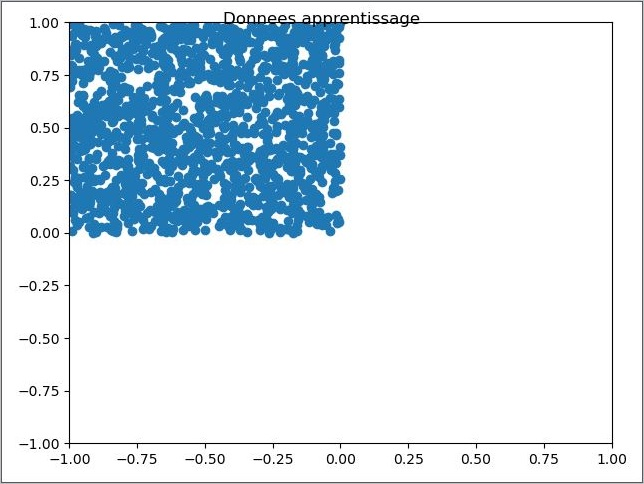
\includegraphics[scale=0.8]{jeu_donnees_1_analyse.JPG}
\captionof{figure}{Jeu de données pour l'analyse}
\label{fig1}
\end{center}


\subsection{Analyse de l'influence du taux d'apprentissage $\eta$}
Lorsque le taux d'apprentissage $\eta$ est élevé, le vecteur de poids des neurones est fortement mis à jour pour chaque entrée présentée. Ils vont donc s'organiser très rapidement, avec une forte mise à jour du vecteur poids à chaque itération, mais la répartition des neurones est instable et brouillonne par rapport au jeu de données d'entrée.\\
En revanche, si le taux d'apprentissage est faible, il va falloir plus d'itérations pour que les vecteurs de poids des neurones soient bien ajustés au jeu de données d'entrée, mais leur répartition sera mieux organisée et collera mieux au jeu de données d'entrée.\\
Les figures ci-dessous présentent les résultats de différentes exécutions, où j'ai changé uniquement le coefficient d'apprentissage $\eta$.\\
La \hyperlink{figure-eta-0.04}{Figure \ref{figure-eta-0.04}} présente le cas où $\eta$ a été fixé à $0.04$, montrant la carte de neurones respectivement au bout de $6`000$ et $30`000$ itérations. \\
De même, la \hyperlink{figure-eta-0.96}{Figure \ref{figure-eta-0.96}} présente le cas où $\eta$ a été fixé à $0.96$, montrant la carte de neurones respectivement au bout de $6`000$ et $30`000$ itérations. \\
En fin d'exécution, l'erreur de quantification vectorielle moyenne est de 0.00446 dans le cas où $\eta = 0.04$, et de 0.00857 dans le cas où $\eta = 0.96$.\\
Ainsi, malgré des coefficients d'apprentissage très différents et un rendu visuel de la carte de neurone différent également, le fait de fixer le taux d'apprentissage très élevé ou très bas n'a pas très fortement impacté la validité des poids de notre réseau de neurone en fin d'exécution, notamment car le nombre d'itération est assez élevé ($N = 30`000$).\\

\begin{figure}[H]
    \centering
    \hypertarget{figure-eta-0.04}{}
    \subfloat[Itération 6`000]{
        \label{figure-eta-0.04-6000}
        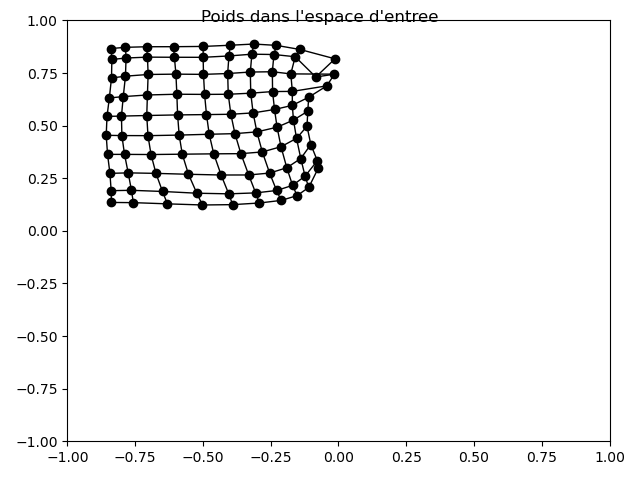
\includegraphics[width=0.5\textwidth]{eta_petit_ite6000.png}
    }
    \subfloat[Itération 30`000]{
        \label{figure-eta-0.04-30000}
        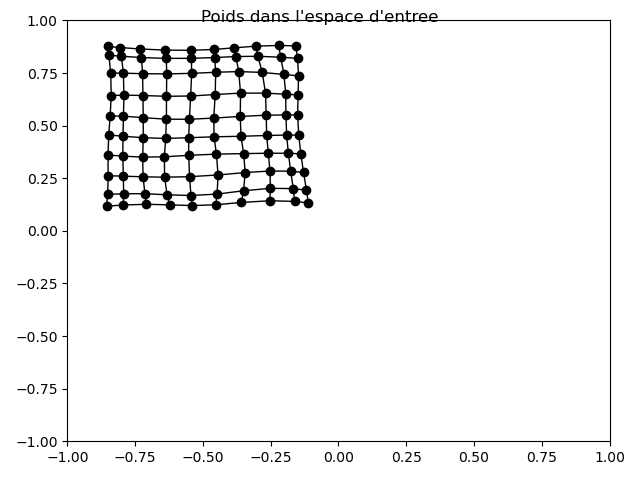
\includegraphics[width=0.5\textwidth]{eta_petit_ite30000.png}
    }
    \caption{Cartes des neurones pour $\eta = 0.04$}
    \label{figure-eta-0.04}
\end{figure}

\begin{figure}[H]
    \centering
    \hypertarget{figure-eta-0.96}{}
    \subfloat[Itération 6`000]{
        \label{figure-eta-0.96-6000}
        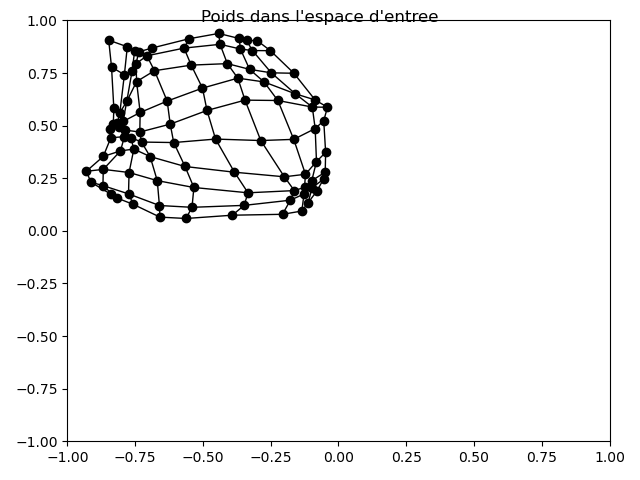
\includegraphics[width=0.5\textwidth]{eta_grand_ite6000.png}
    }
    \subfloat[Itération 30`000]{
        \label{figure-eta-0.96-30000}
        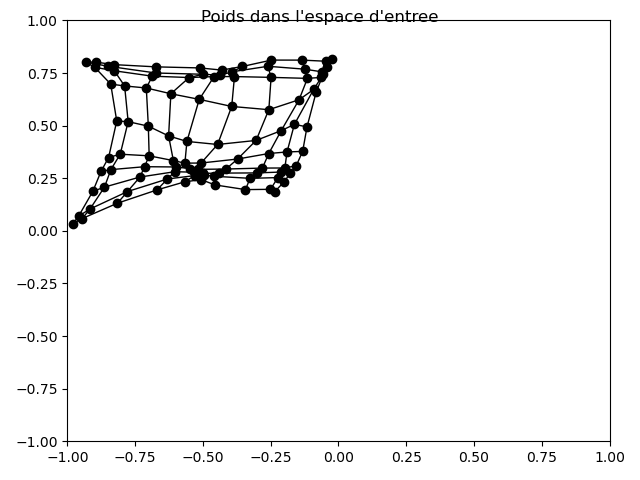
\includegraphics[width=0.5\textwidth]{eta_grand_ite30000.png}
    }
    \caption{Cartes des neurones pour $\eta = 0.96$}
    \label{figure-eta-0.96}
\end{figure}

\subsection{Analyse de l'influence de la largeur de voisinage $\sigma$}

Pour cette analyse de l'influence de $\sigma$, j'ai fixé le taux d'apprentissage $\eta = 0.05$.\\
Lorsque la largeur de voisinage $\sigma$ est élevée, le vecteur de poids des neurones relativement éloignés du neurone gagnant est plus fortement mis à jour pour chaque entrée présentée que si $\sigma$ est faible. Avec une grande largeur de voisinage $\sigma$, les neurones vont ainsi avoir tendance à se regrouper autour du neurone gagnant, puisqu'ils sont très influencés par lui. Cela donne donc des cartes de neurones assez resserrés après exécution.\\
En revanche, si le taux d'apprentissage est faible, les neurones même proches du neurone gagnant ont leurs poids très peu mis à jour, si bien que le neurone gagnant va avoir tendance à s'éloigner tout seul. Les neurones vont donc se déplacer beaucoup plus lentement, et vont être répartis de manière plus éparse.\\
Les figures ci-dessous présentent les résultats de différentes exécutions, où j'ai changé uniquement le coefficient d'apprentissage $\sigma$.\\
La \hyperlink{figure-sigma-0.8}{Figure \ref{figure-sigma-0.8}} présente le cas où $\sigma$ a été fixé à $0.8$, valeur assez basse, montrant la carte de neurones respectivement au bout de $6`000$ et $30`000$ itérations. \\
De même, la \hyperlink{figure-sigma-4}{Figure \ref{figure-sigma-4}} présente le cas où $\sigma$ a été fixé à $4$, valeur assez élevée, montrant la carte de neurones respectivement au bout de $6`000$ et $30`000$ itérations. \\
Enfin, la \hyperlink{figure-sigma-extremes}{Figure \ref{figure-sigma-extremes}} présente la carte de neurones après $30`000$ itérations, respectivement pour $\sigma = 0.2$ et $\sigma = 15$, deux valeurs extrêmes.\\
En fin d'exécution, l'erreur de quantification vectorielle moyenne est de 0.00304 dans le cas où $\sigma = 0.8$, et de 0.04155 dans le cas où $\sigma = 4$. Pour $\sigma = 0.2$, l'erreur de quantification vectorielle moyenne est de 0.01167, tandis que pour $\sigma = 15$ elle est de 0.1498.\\
Comme pour l'analyse de l'influence du taux d'apprentissage $\eta$, on se rend compte que malgré des largeurs de voisinage $\sigma$ très différentes et un rendu visuel de la carte de neurone différent également, le fait de fixer la largeur de voisinage $\sigma$ raisonnablement élevée ou raisonnablement basse n'a pas très fortement impacté la validité des poids de notre réseau de neurone en fin d'exécution, notamment car le nombre d'itération est assez élevé ($N = 30`000$).\\
Néanmoins, même si, malgré son apparence semblant prouver le contraire, la valeur extrême de $\sigma = 0.2$ n'a pas trop dégradé l'erreur de quantification vectorielle moyenne, la valeur de $\sigma = 15$ a quand à elle totalement dégradé la validité des poids de notre réseau de neurone, et le placement de ces derniers est très mauvais.\\


\begin{figure}[H]
    \centering
    \hypertarget{figure-sigma-0.8}{}
    \subfloat[Itération 6`000]{
        \label{figure-sigma-0.8-6000}
        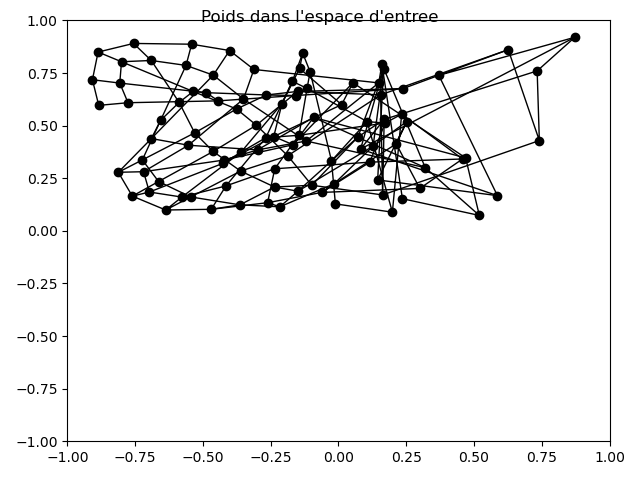
\includegraphics[width=0.5\textwidth]{sigma_0.8_ite6000.png}
    }
    \subfloat[Itération 30`000]{
        \label{figure-sigma-0.8-30000}
        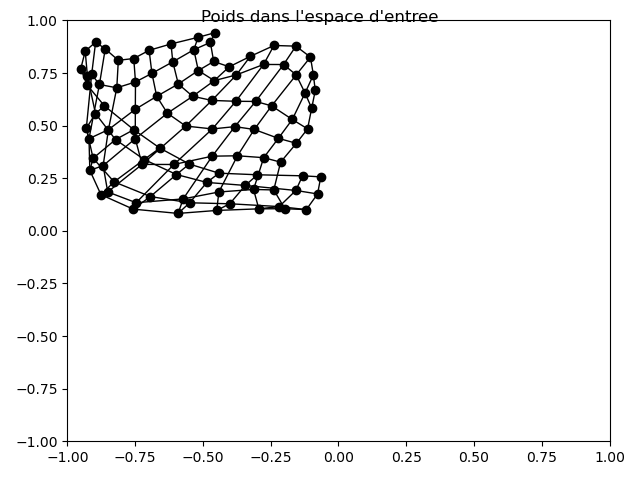
\includegraphics[width=0.5\textwidth]{sigma_0.8_ite30000.png}
    }
    \caption{Cartes des neurones pour $\sigma = 0.8$}
    \label{figure-sigma-0.8}
\end{figure}


\begin{figure}[H]
    \centering
    \hypertarget{figure-sigma-4}{}
    \subfloat[Itération 6`000]{
        \label{figure-sigma-4-6000}
        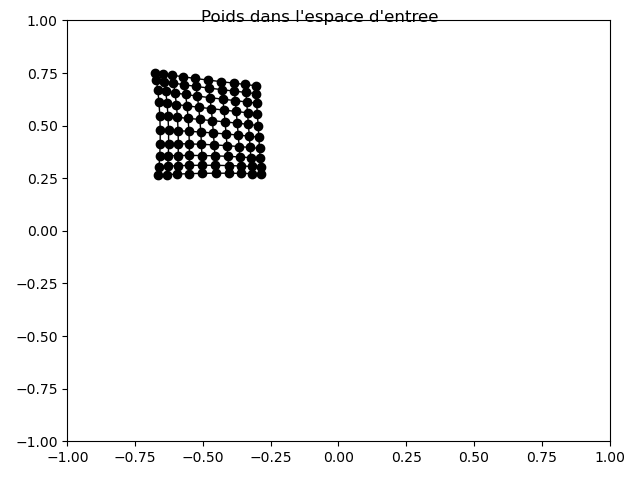
\includegraphics[width=0.5\textwidth]{sigma_4_ite6000.png}
    }
    \subfloat[Itération 30`000]{
        \label{figure-sigma-4-30000}
        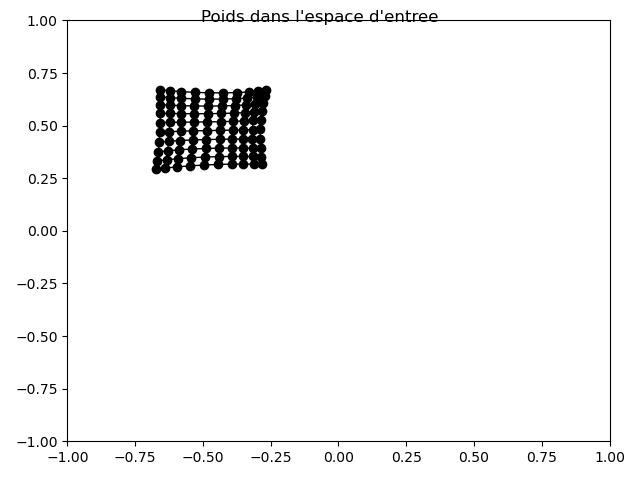
\includegraphics[width=0.5\textwidth]{sigma_4_ite30000.png}
    }
    \caption{Cartes des neurones pour $\sigma = 4$}
    \label{figure-sigma-4}
\end{figure}


\begin{figure}[H]
    \centering
    \hypertarget{figure-sigma-extremes}{}
    \subfloat[$\sigma = 0.2$, Itération 30`000]{
        \label{figure-sigma-extremes-0.2}
        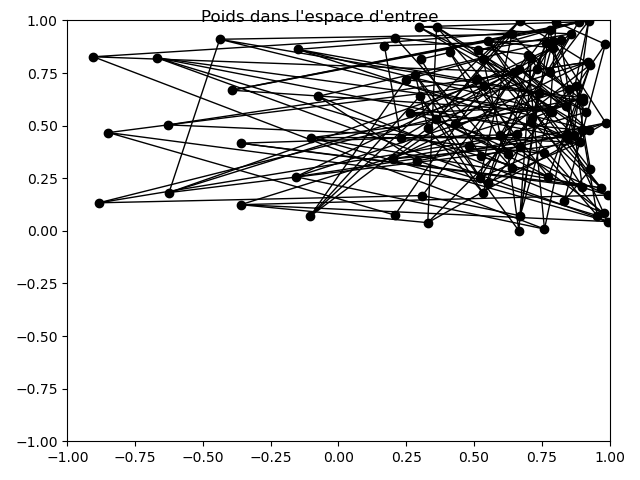
\includegraphics[width=0.5\textwidth]{extreme_sigma_0.2.png}
    }
    \subfloat[$\sigma = 15$, Itération 30`000]{
        \label{figure-sigma-extremes-15}
        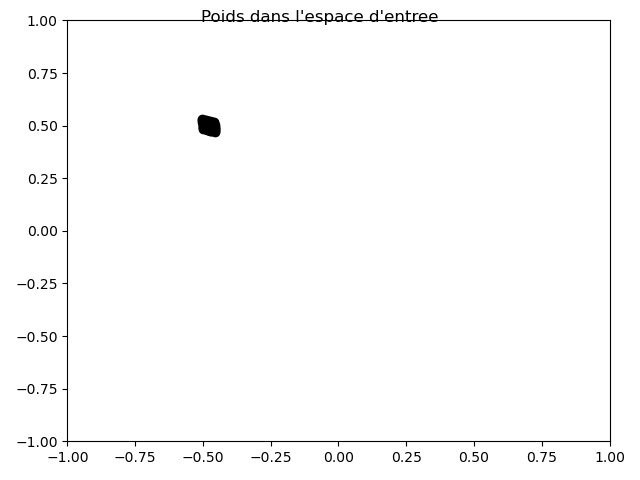
\includegraphics[width=0.5\textwidth]{extreme_sigma_15.png}
    }
    \caption{Cartes des neurones pour des valeurs de $\sigma$ extrêmes}
    \label{figure-sigma-extremes}
\end{figure}


\subsection{Analyse de l'influence du nombre de pas d'apprentissage $N$}

Ici, j'ai travaillé avec un taux d'apprentissage $\eta = 0.05$ et une largeur de voisinage $\sigma = 1.4$.\\
Le nombre de pas d'apprentissage joue un rôle clé : si celui-ci est trop faible, les neurones n'auront pas le temps d'apprendre car trop peu de données leur auront été présentées.\\
Si le taux d'apprentissage $\eta$ était plus élevé, on pourrait diminuer quelque peu $N$, cependant au détriment de l'erreur de quantification vectorielle.\\
Cependant, si le nombre de pas d'apprentissage $N$ est trop élevé, le temps de processing augmente drastiquement, et l'amélioration du résultat est inexistante, ou du moins pas à la hauteur des ressources supplémentaires engagées lorsqu'on augmente fortement $N$.\\
La \hyperlink{figure-N-normales}{Figure \ref{figure-N-normales}} présente deux cas de valeurs de $N$ raisonnables (pas trop élevées), respectivement $N = 3`000$ et $N = 30`000$. Le calcul pour $N = 3`000$ prend de l'ordre d'une dizaine de secondes, tandis que celui pour $N = 30`000$ prend approximativement une bonne minute. L'erreur de quantification vectorielle moyenne dans le premier cas est de 0.006627, tandis que dans le deuxième cas elle est de 0.004796. On voit donc qu'il y a eu une amélioration entre les deux cas, même si elle n'est pas flagrante. En revanche, la répartition des neurones sur la carte semble bien meilleure dans le deuxième cas.\\
La \hyperlink{figure-N-extremes}{Figure \ref{figure-N-extremes}} quand à elle présente 3 cas de valeurs de $N$ 'extrêmes', respectivement $N = 300$, $N = 300`000$ et $N = 3`000`000$. Dans le premier cas, l'erreur de quantification vectorielle moyenne est vraiment mauvaise par rapport aux autres valeurs de $N$ testées, avec 0.032305, ce qui est corroboré par l'aspect de la carte de neurones, qui ne correspond que très peu aux données. Néanmoins, il ne m'a fallu qu'une seconde pour faire le processing.\\
Pour $N = 300`000$, l'erreur de quantification vectorielle moyenne est de 0.004739, ce qui ne représente qu'une très faible amélioration par rapport à $N = 30`000$, alors qu'il m'a fallu une dizaine de minute pour avoir le résultat. On voit d'ailleurs que la carte de neurones est très similaire à celle de $N = 30`000$. \\
De même, pour $N = 3`000`000$, l'erreur de quantification vectorielle moyenne est de 0.004349, ce qui ne représente pas une forte amélioration au vu des deux heures qu'il aura fallu à mon ordinateur pour faire le calcul ! Et la carte de neurones ressemble énormément à celles de $N = 30`000$ et $N = 300`000$.\\
Il faut donc paramétrer le nombre de pas d'apprentissage $N$ à une valeur assez élevée pour obtenir de bons résultats, sans toutefois régler le paramètre $N$ trop élevé, cela va simplement ralentir l'exécution sans notablement améliorer le résultat.

\begin{figure}[H]
    \centering
    \hypertarget{figure-N-normales}{}
    \subfloat[$N = 3`000$]{
        \label{figure-N-normales-3000}
        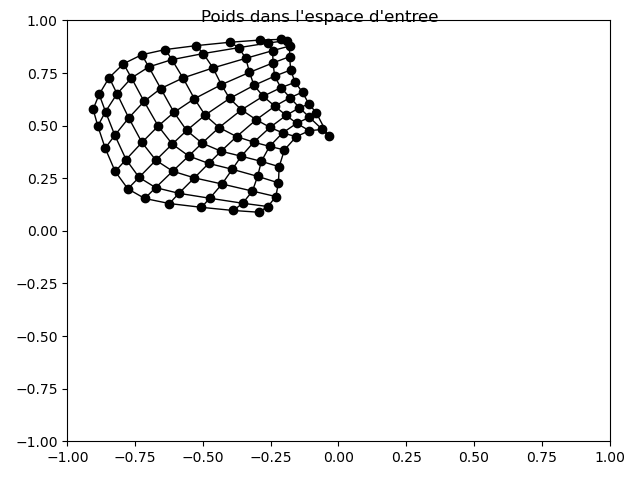
\includegraphics[width=0.5\textwidth]{N_3000_petit.png}
    }
    \subfloat[$N = 30`000$]{
        \label{figure-N-normales-30000}
        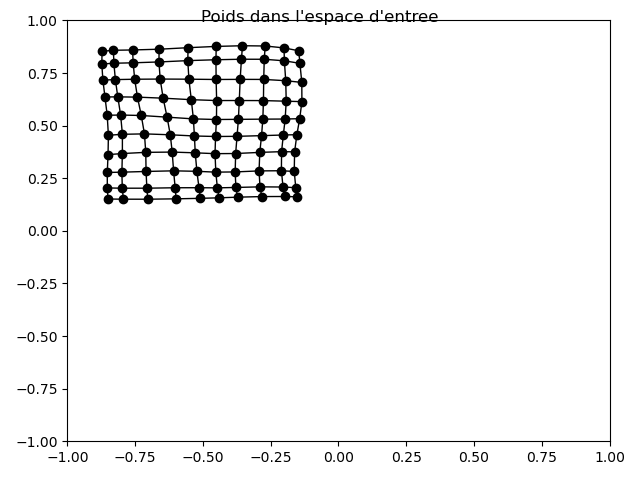
\includegraphics[width=0.5\textwidth]{N_30000_normal.png}
    }
    \caption{Cartes des neurones pour des valeurs de $N$ raisonnablement normales}
    \label{figure-N-normales}
\end{figure}

\begin{figure}[H]
    \centering
    \hypertarget{figure-N-extremes}{}
    \subfloat[$N = 300$]{
        \label{figure-N-extremes-300}
        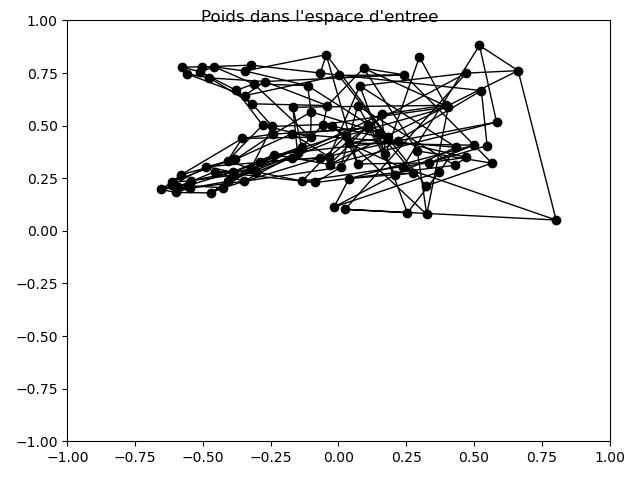
\includegraphics[width=0.33\textwidth]{N_300_minuscule.png}
    }
    \subfloat[$N = 300`000$]{
        \label{figure-N-extremes-300000}
        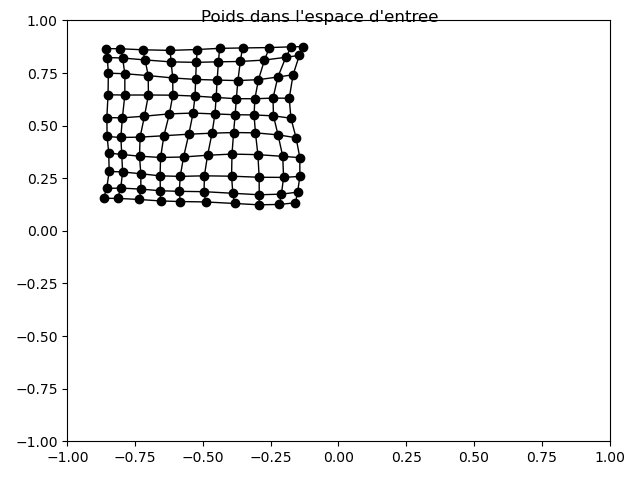
\includegraphics[width=0.33\textwidth]{N_300000_grand.png}
    }
    \subfloat[$N = 3`000`000$]{
        \label{figure-N-extremes-3000000}
        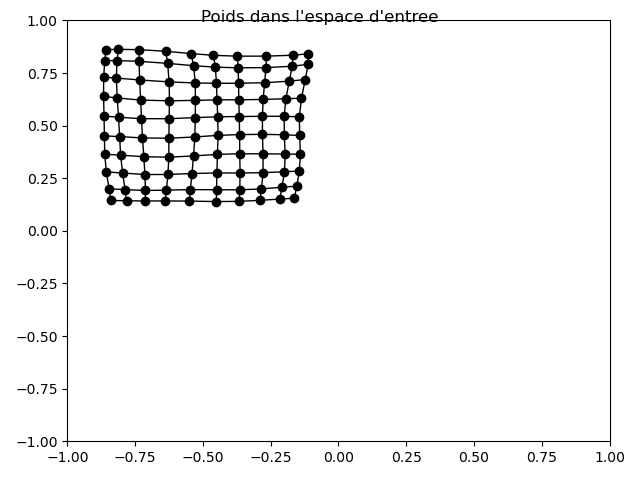
\includegraphics[width=0.33\textwidth]{N_3000000_immense.png}
    }
    \caption{Cartes des neurones pour des valeurs de $N$ extrêmes}
    \label{figure-N-extremes}
\end{figure}


\subsection{Analyse de l'influence des caractéristiques de la carte}

Pour cette analyse, j'ai travaillé avec un taux d'apprentissage $\eta = 0.05$, une largeur de voisinage $\sigma = 1.4$ ainsi qu'un nombre de pas d'apprentissage $N=30`000$.\\

\subsubsection{Analyse de l'influence de la taille de la carte}

L'augmentation de la taille de la carte (du nombre de neurones, donc de leur densité dans la carte) améliore le partitionnement de l'espace d'entrée. L'erreur de quantification vectorielle moyenne est donc plus faible. \\
Ceci va donc permettre d'avoir des neurones apprenant mieux les espaces d'entrées desquels ils sont proches. Cependant, cela a un coût : le temps de processing.\\
Ainsi, si on diminue le nombre de neurones sur la carte, l'apprentissage sera moins bon, mais beaucoup plus rapide.\\
La \hyperlink{figure-taille-carte}{Figure \ref{figure-taille-carte}} présente deux cartes de neurones, de tailles respectives 4 par 4 et 20 par 20 neurones, qui ont appris sur le même jeu de données et pendant le même nombre d'itérations ($N = 30`000$). Pour la carte de 16 neurones, l'erreur de quantification vectorielle moyenne est de 0.04539, tandis qu'elle n'est que de 0.00101 pour la carte de 400 neurones.\\
Cependant, la carte de 16 neurones a nécessité une dizaine de secondes de calcul, tandis que celle de 400 neurones a nécessité 6 minutes de processing.\\
La précision obtenue avec une carte plus dense n'a donc rien a voir avec celle d'une carte de plus petite taille, mais s'il n'est pas nécessaire d'avoir une très grande précision, autant s'abstenir d'utiliser trop de neurones et de rallonger ainsi le temps de calcul.

\begin{figure}[H]
    \centering
    \hypertarget{figure-taille-carte}{}
    \subfloat[4*4 neurones, Itération 30`000]{
        \label{figure-taille-carte_4x4}
        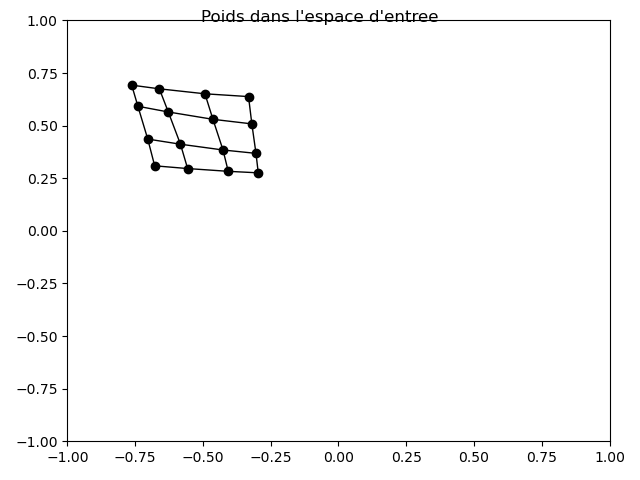
\includegraphics[width=0.5\textwidth]{4x4_ite30000.png}
    }
    \subfloat[20*20 neurones, Itération 30`000]{
        \label{figure-taille-carte_20x20}
        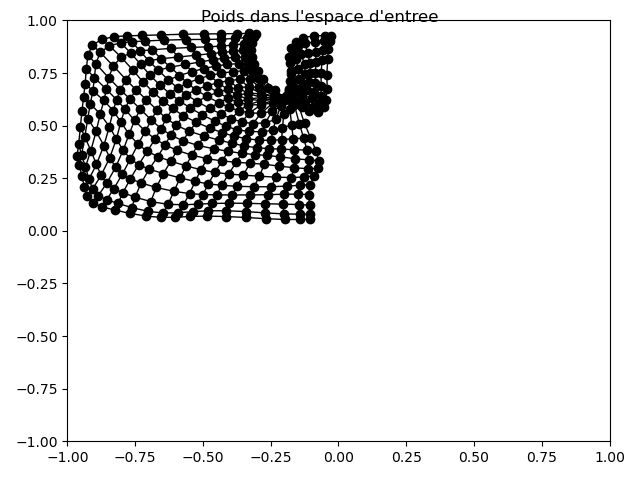
\includegraphics[width=0.5\textwidth]{20x20_ite30000.png}
    }
    \caption{Cartes de neurones de différentes tailles}
    \label{figure-taille-carte}
\end{figure}

\subsubsection{Analyse de l'influence de la forme de la carte}

Pour cette analyse, j'ai toujours utilisé une carte de 160 neurones, mais j'ai fait varier la forme de celle-ci.\\
La forme de la carte influe sur la manière dont les neurones vont évoluer en fonction des données d'entrée. Moins la carte a la forme du jeu de données, plus il va être difficile de bien apprendre des données d'entrée.\\
La \hyperlink{figure-forme-comme-data}{Figure \ref{figure-forme-comme-data}} présente deux cartes de neurones relativement adaptées aux données d'entrées, de dimensions respectives 10 par 16 et 8 par 20 neurones.\\
La \hyperlink{figure-forme-differente-data}{Figure \ref{figure-forme-differente-data}} présente deux cartes de neurones dont la forme n'est pas bien adaptée pour les données d'entrée, de dimensions respectives 5 par 32 et 4 par 40 neurones.\\
Enfin, la \hyperlink{figure-forme-inadapte-data}{Figure \ref{figure-forme-inadapte-data}} présente deux cartes vraiment inadaptées au jeu de données, de dimensions respectives 2 par 80 et 1 par 160 neurones.\\
Les deux cartes adaptées représentent plutôt bien les données d'entrées, même si celle de dimensions 8 par 20 a déjà une forme bizarre. Leurs erreurs de quantification vectorielle moyenne sont 0.00309 pour la 10 par 16 et 0.00388 pour la 8 par 20.\\
Bizarrement, la carte 5 par 32 a une erreur de quantification vectorielle moyenne meilleure que celle de 8 par 20 : 0.00364, alors que la 4 par 40 est loin avec 0.00419.\\
Enfin, la carte 2 par 80 a une erreur de quantification vectorielle moyenne de 0.00403, et la 1 par 160 a la deuxième meilleure valeur, soit 0.00327.\\
J'ai pu identifier qu'il aurait fallu un plus grand nombre de pas d'apprentissage ($N$) pour les cartes de forme inadaptée (comme la 1 par 160) pour qu'elles apprennent mieux et représentent mieux les données d'entrée.\\
J'ai également déduis que celles qui ont une forme mal adaptée, comme la 8 par 20, ne donnent pas de résultats probants, alors que celles ayant des formes inadaptées en théorie, mais plus 'malléable' car étant presque des chaînes (par exemple 1 par 160) peuvent donner des résultats intéressants car elles peuvent vraiment s'adapter au jeu de données.\\
Le temps de processing n'a pas ou peu varié selon la forme, c'est le nombre de neurones qui influence fortement, pas leur organisation.

\begin{figure}[H]
    \centering
    \hypertarget{figure-forme-comme-data}{}
    \subfloat[10*16 neurones, Itération 30`000]{
        \label{figure-forme-comme-data_10x16}
        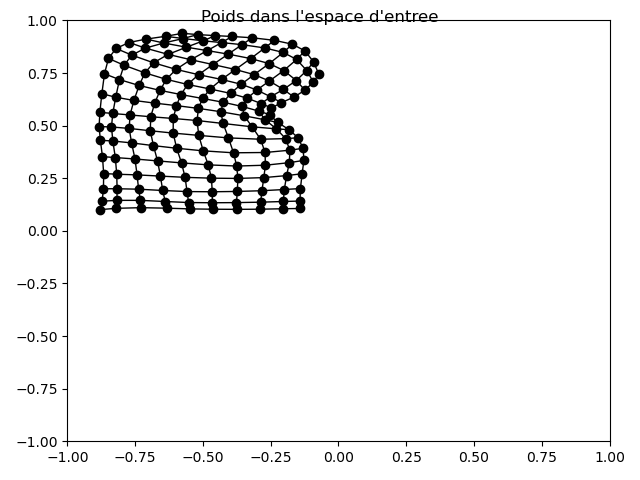
\includegraphics[width=0.5\textwidth]{10x16_ite30000.png}
    }
    \subfloat[8*20 neurones, Itération 30`000]{
        \label{figure-forme-comme-data_8x20}
        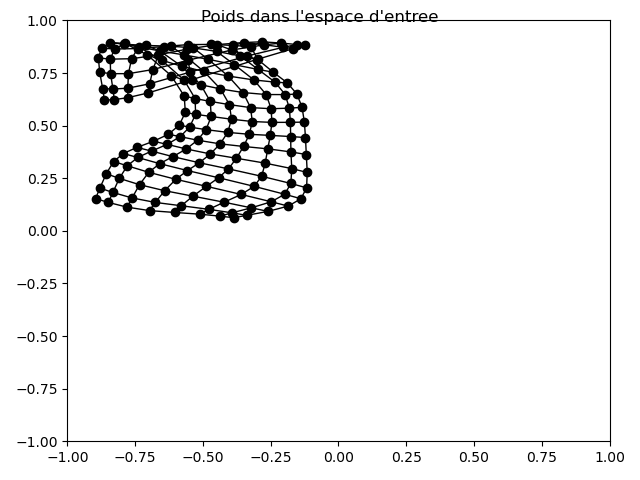
\includegraphics[width=0.5\textwidth]{8x20_ite30000.png}
    }
    \caption{Cartes de neurones de forme assez similaire aux données}
    \label{figure-forme-comme-data}
\end{figure}

\begin{figure}[H]
    \centering
    \hypertarget{figure-forme-differente-data}{}
    \subfloat[5*32 neurones, Itération 30`000]{
        \label{figure-forme-differente-data_5x32}
        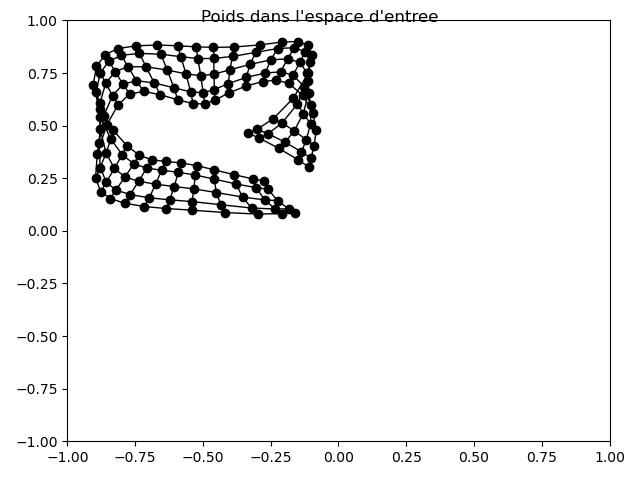
\includegraphics[width=0.5\textwidth]{5x32_ite30000.png}
    }
    \subfloat[4*40 neurones, Itération 30`000]{
        \label{figure-forme-differente-data_4x40}
        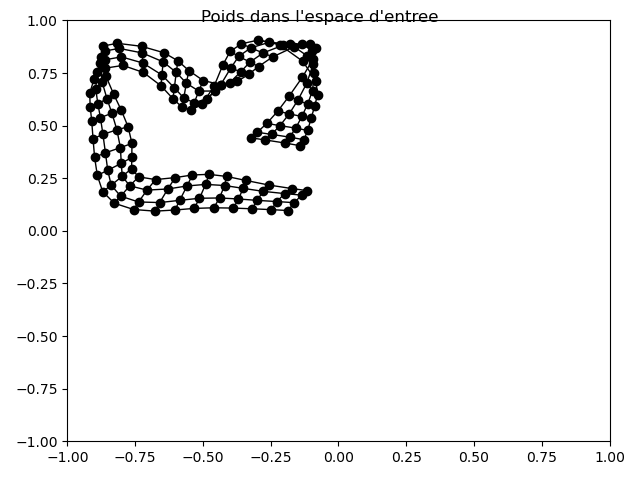
\includegraphics[width=0.5\textwidth]{4x40_ite30000.png}
    }
    \caption{Cartes de neurones de forme différente des données}
    \label{figure-forme-differente-data}
\end{figure}

\begin{figure}[H]
    \centering
    \hypertarget{figure-forme-inadapte-data}{}
    \subfloat[2*80 neurones, Itération 30`000]{
        \label{figure-forme-inadapte-data_2x80}
        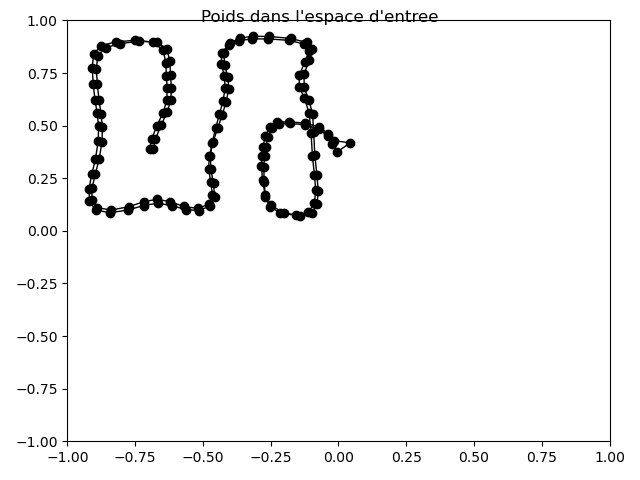
\includegraphics[width=0.5\textwidth]{2x80_ite30000.png}
    }
    \subfloat[1*160 neurones, Itération 30`000]{
        \label{figure-forme-inadapte-data_1x160}
        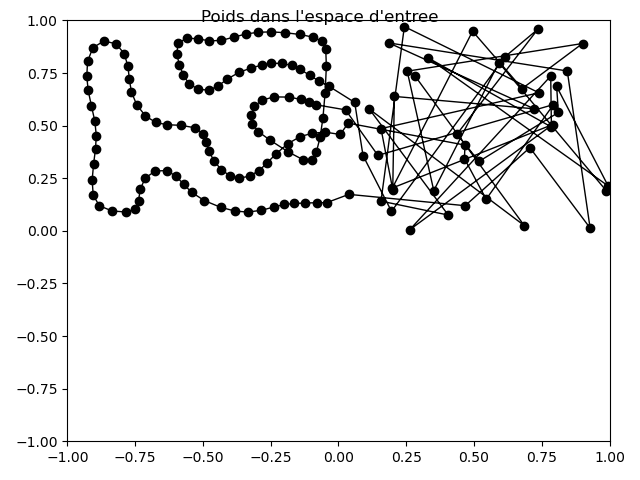
\includegraphics[width=0.5\textwidth]{1x160_ite30000.png}
    }
    \caption{Cartes de neurones de forme inadaptée aux données}
    \label{figure-forme-inadapte-data}
\end{figure}


\subsection{Analyse de l'influence des caractéristiques du jeu de données}

Pour cette analyse, j'ai travaillé avec un taux d'apprentissage $\eta = 0.05$, une largeur de voisinage $\sigma = 1.4$ ainsi qu'un nombre de pas d'apprentissage $N=30`000$. Ma carte de neurones fait 10 par 10 neurones.\\
De la même manière que pour l'analyse précédente sur les caractéristiques de la carte de neurones, si le jeu de données change et n'est plus adapté à la carte, il va être difficile de faire un apprentissage correct.\\
Si la forme des données est incompatible avec celle de la carte, les neurones vont se déplacer au mieux pour représenter les données mais le résultat peut ne pas être fidèle voire être trompeur.\\
La \hyperlink{figure-sample-1}{Figure \ref{figure-sample-1}} présente le résultat du processing avec les caractéristiques décrites ci-dessus sur le jeu de données 1.\\
La \hyperlink{figure-sample-2}{Figure \ref{figure-sample-2}} présente le résultat du processing avec les caractéristiques décrites ci-dessus sur le jeu de données 2.\\
La \hyperlink{figure-sample-3}{Figure \ref{figure-sample-3}} présente le résultat du processing avec les caractéristiques décrites ci-dessus sur le jeu de données 3.\\
La \hyperlink{figure-sample-4}{Figure \ref{figure-sample-4}} présente le résultat du processing avec les caractéristiques décrites ci-dessus sur un jeu de données de forme triangulaire pour lequel je me suis fait aider par un camarade.\\
Comme depuis le début, pour le sample 1, pas de soucis, le réseau de neurone a bien appris, et l'erreur de quantification vectorielle moyenne est de 0.00477. Cependant, ce n'est pas le cas pour tous les samples.\\
En effet, les samples 2 et 3 n'ont pas une forme carrée comme la carte de neurones, si bien que l'erreur de quantification vectorielle moyenne pour chacun de ces samples est respectivement 0.01541 et 0.01367.\\
En revanche, pour le sample 4, elle est de 0.00233, ce qui est une bonne valeur. On peut remarquer que certaines formes sont compatibles entre elles, mais d'autres non. Par exemple, la carte rectangulaire représente bien le jeu de données triangulaire, mais pour les deux jeux de données se situants dans plusieurs quadrants, la représentation est plus hasardeuse, moins fidèle aux données d'entrée.\\
Peut-être qu'ici une carte de la bonne forme ou alors une carte de type ruban (1 ou 2 noeuds de large sur une grande longueur) avec un plus grand nombre de pas d'apprentissage $N$ aurait permis de mieux apprendre.


\begin{figure}[H]
    \centering
    \hypertarget{figure-sample-1}{}
    \subfloat[Sample de données 1]{
        \label{figure-sample-1-data}
        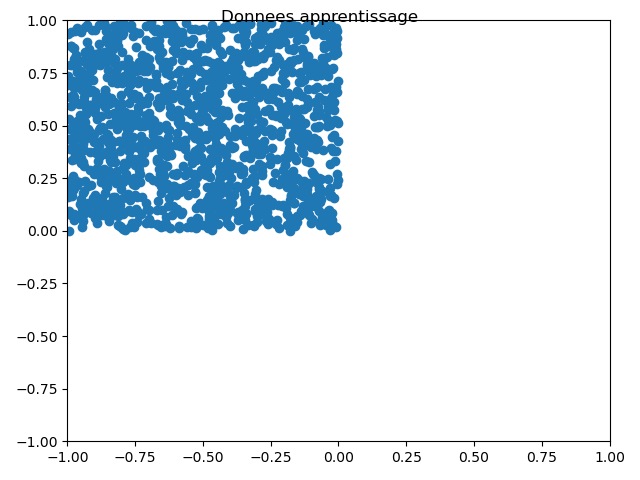
\includegraphics[width=0.5\textwidth]{sample1.png}
    }
    \subfloat[Résultat sur le sample 1, Itération 30`000]{
        \label{figure-sample-1-result}
        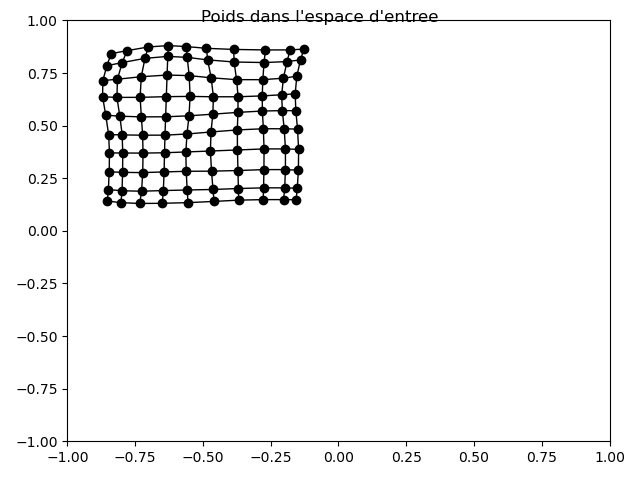
\includegraphics[width=0.5\textwidth]{sample1_ite30000.png}
    }
    \caption{Résultat avec le sample 1}
    \label{figure-sample-1}
\end{figure}

\begin{figure}[H]
    \centering
    \hypertarget{figure-sample-2}{}
    \subfloat[Sample de données 2]{
        \label{figure-sample-2-data}
        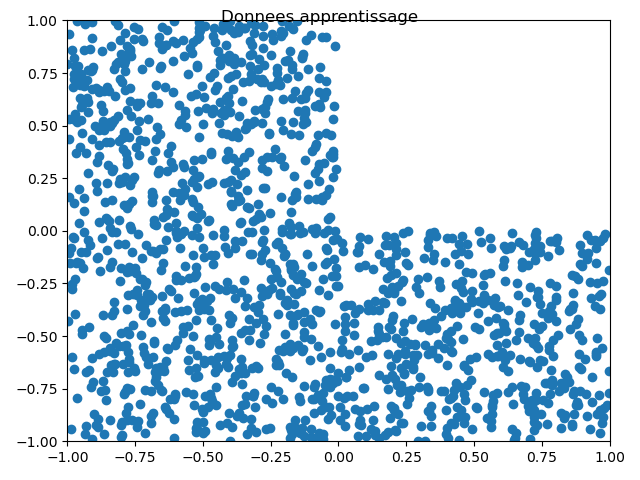
\includegraphics[width=0.5\textwidth]{sample2.png}
    }
    \subfloat[Résultat sur le sample 2, Itération 30`000]{
        \label{figure-sample-2-result}
        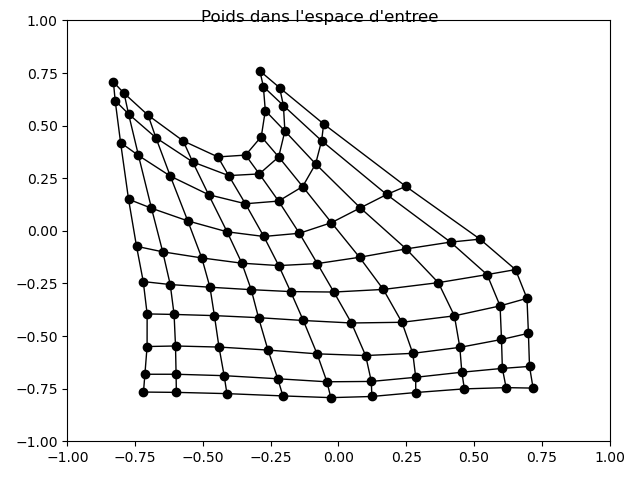
\includegraphics[width=0.5\textwidth]{sample2_ite30000.png}
    }
    \caption{Résultat avec le sample 2}
    \label{figure-sample-2}
\end{figure}

\begin{figure}[H]
    \centering
    \hypertarget{figure-sample-3}{}
    \subfloat[Sample de données 3]{
        \label{figure-sample-3-data}
        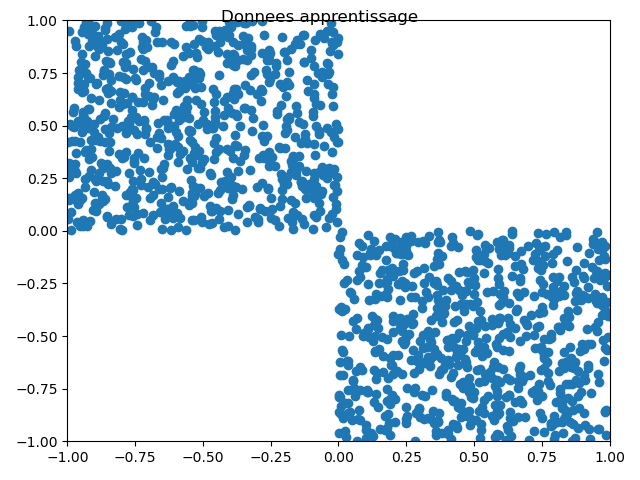
\includegraphics[width=0.5\textwidth]{sample3.png}
    }
    \subfloat[Résultat sur le sample 3, Itération 30`000]{
        \label{figure-sample-3-result}
        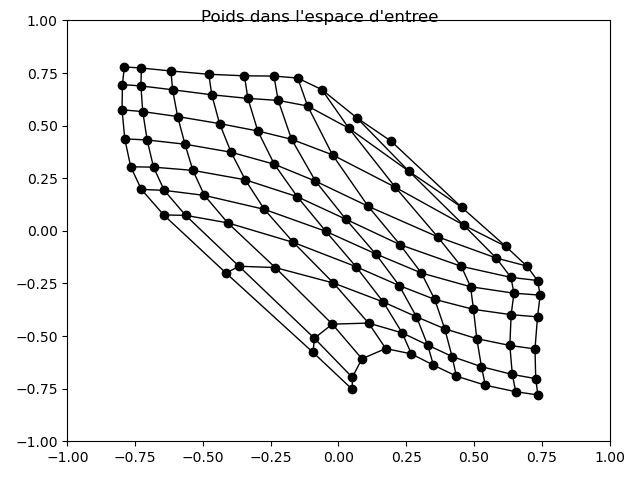
\includegraphics[width=0.5\textwidth]{sample3_ite30000.png}
    }
    \caption{Résultat avec le sample 3}
    \label{figure-sample-3}
\end{figure}

\begin{figure}[H]
    \centering
    \hypertarget{figure-sample-4}{}
    \subfloat[Sample de données 4]{
        \label{figure-sample-4-data}
        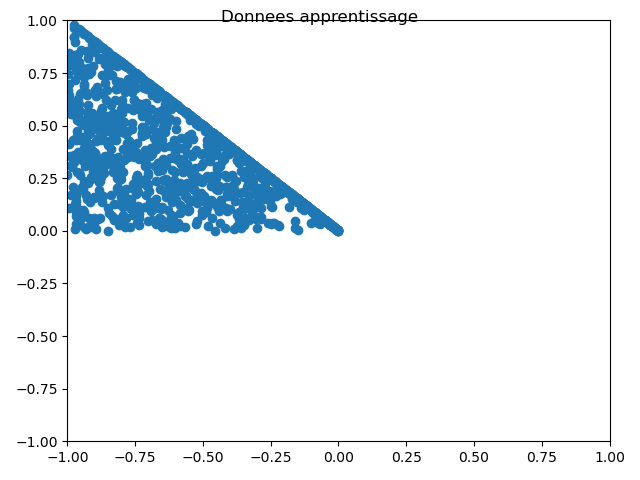
\includegraphics[width=0.5\textwidth]{sample4.png}
    }
    \subfloat[Résultat sur le sample 4, Itération 30`000]{
        \label{figure-sample-4-result}
        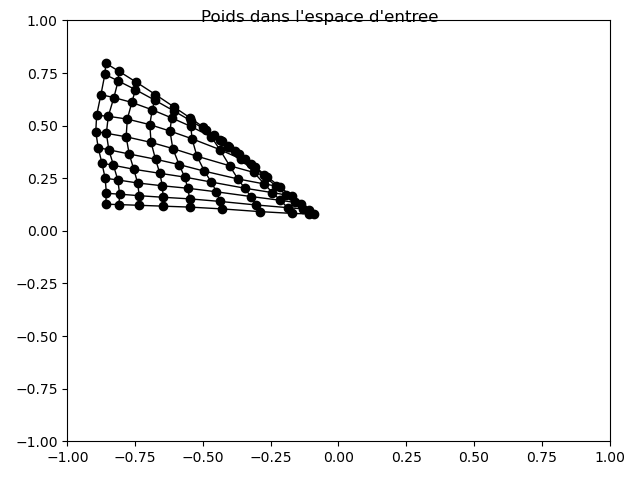
\includegraphics[width=0.5\textwidth]{sample4_ite30000.png}
    }
    \caption{Résultat avec le sample 4}
    \label{figure-sample-4}
\end{figure}

\section{Bras robotique}


\subsection{Comment prédire la position ?}
Une fois la carte apprise, il va falloir déterminer une équation à partir des poids des neurones, permettant de passer du vecteur de commande motrice $\theta$ au vecteur de position spatiale $x$ et inversement.\\
Ceci nous permettra à la fois de déterminer la commande nécessaire pour atteindre une position donnée sachant la position actuelle, ainsi que de déterminer la position spatiale résultante d'une commande motrice donnée connaissant la position spatiale actuelle.

\subsection{Modèle proche}
Cette méthode d'apprentissage, consistant à apprendre une entrée et une sortie pour être capable de retrouver l'une à partir de l'autre ou d'une partie de l'autre se rapproche du modèle de Hopfield.\\
Le modèle de Hopfield s'apparente à un apprentissage par coeur. Son principal avantage est que tant que l'entrée que nous lui donnons est assez similaire à l'entrée que nous avions en apprentissage, il va pouvoir nous reconstruire la sortie souhaitée. Son inconvénient majeur est le nombre colossal de neurones qu'il nécessite, plus de 7 fois plus de neurones que la taille de l'entrée à mémoriser par coeur. De plus, rien ne garantit qu'il ne peut pas y avoir un autre bassin d'attraction involontaire qui pourrait biaiser la reconstitution de la sortie depuis l'entrée ou de l'entrée depuis la sortie.

\subsection{Prédiction de la position spatiale uniquement}
Pour prédire uniquement la position spatiale en fonction du vecteur de commande motrice, nous aurions pu utiliser le modèle Perceptron multi-couches, qui permet de s'affranchir de la limitation linéaire du Perceptron standard. Le problème est qu'il n'y a pas de convergence garantie.


\end{document}
